% chktex-file 13

\documentclass{article}
\usepackage{amsmath}
\usepackage{hyperref}
\usepackage{xcolor}
\usepackage{ulem}
\usepackage{graphicx}
\usepackage[margin=0.75in]{geometry}
\usepackage{adjustbox}

\graphicspath{ {./images/} }

\definecolor{darkblue}{rgb}{0, 0, 20}

\hypersetup{
    colorlinks=true,
    urlcolor=darkblue,
    linkcolor=blue,
    filecolor=magenta,
    citecolor=blue,
}

\title{HandDAGT: A Denoising Adaptive Graph Transformer for 3D Hand Pose Estimation}
\author{Wencan Cheng, Eunji Kim, Jong Hwan Ko}
\date{}
\setlength{\parindent}{0pt}

\begin{document}

\maketitle

\begin{center}\textbf{Accepted for ECCV 2024 (\href{https://arxiv.org/pdf/2407.20542}{Paper}) (\href{https://github.com/cwc1260/HandDAGT}{GitHub})}\end{center}

This paper proposes a transformer-based architecture that uses the image depth map and hand point cloud to predict the 3D hand joint locations. The depth map and point cloud are used to generate keypoint embeddings and 3D local patches, which are then passed to the graph transformer as queries and keys to determine the hand keypoints. Also, random noise is incorporated in the training process to improve the model's noise and occlusion handling.

\section*{Motivation}

Existing graph methods in 3D hand pose estimation use static graphs which are unable to capture dynamic kinematic relations between joints in occluded scenarios. Also, self-occlusion and hand-object occlusion are major challenges for current methods.

\begin{center}
    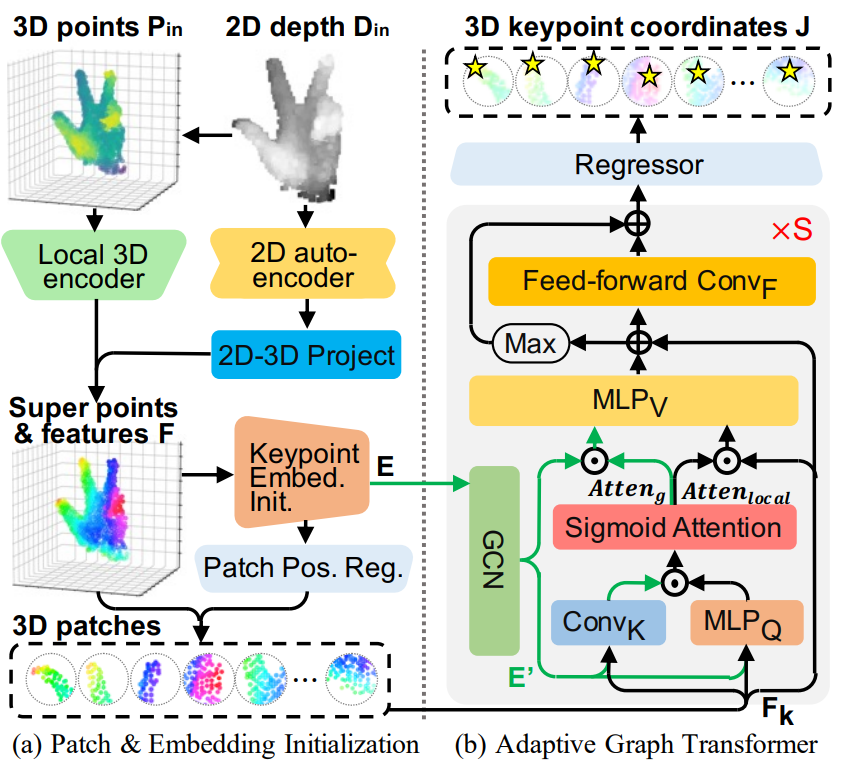
\includegraphics[scale=0.4]{handdagt-1.png}
\end{center}

\section*{Method}

\begin{enumerate}
    \item \textbf{Super Points Generation}
    
    A convolutional layer is used to extract a subsampled 3D super point set from the points in the hand point cloud. The depth is fed into a ConvNeXt-based autoencoder to generate a 2D local visual feature map. The 2D point features are then projected to 3D and concatenated to the super points.

    \item \textbf{Initialization of Keypoint Embedding and Patch Position}
    
    The super points are fed through two convolutional layers to generate 3D global vectors. The 3D global vectors are then replicated $J$ times and then passed through a three-layer bias-induced layer to generate the $J$ keypoint embeddings. The embeddings are linear transformed to project them into the 3D space as the initial keypoint locations. The $K$-nearest super points around each point form its 3D point patch.

    \item \textbf{Adaptive Graph Transformer Decoder}

     The keypoint embeddings are refined using a GCN to incorporate kinematic relationships between keypoints. The 3D patches and enhanced keypoint embeddings are passed through the sigmoid attention mechanism to dynamically balance local attention for visible keypoints and kinematic attention for occluded ones. The updated embeddings are aggregated using residual connections (to ensure original geometric details are preserved) and a point set convolution, and then a linear transformation projects them to the 3D keypoint coordinates.
\end{enumerate}

\begin{center}
    \adjustbox{valign=m}{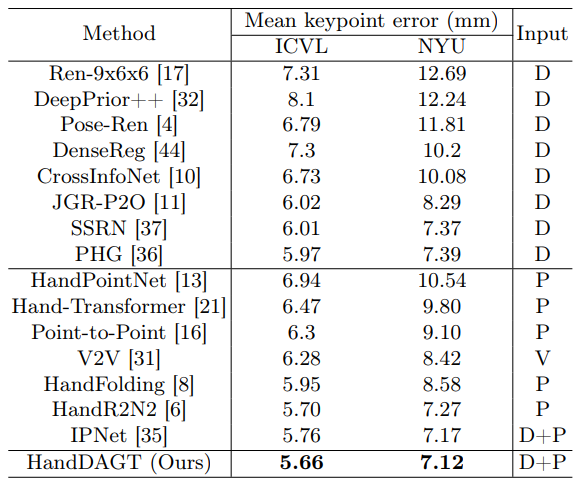
\includegraphics[scale=0.5]{handdagt-2.png}}
    \adjustbox{valign=m}{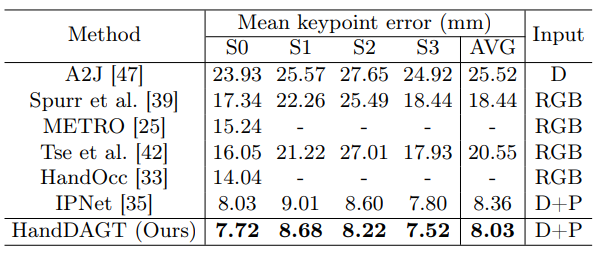
\includegraphics[scale=0.5]{handdagt-3.png}}
\end{center}

\section*{Limitations}

\begin{enumerate}
    \item The model can't process interacting hands (multi-hand interaction)
    \item This method requires redundant computation due to the 2D feature extraction. They state that possible solutions include bidirectional learning and developing a lightweight 2D model.
\end{enumerate}
\end{document}